\clearpage
\subsection{Results and Analysis}
The first test was carried out considering only the diffusive term, in a square plate at a certain temperature, where a peak with a higher temperature is introduced. In this case, it was tested by writing it in two ways: using matrix-vector operations (1) and matrix-matrix operations (2).
\begin{figure}[H]
    \centering
    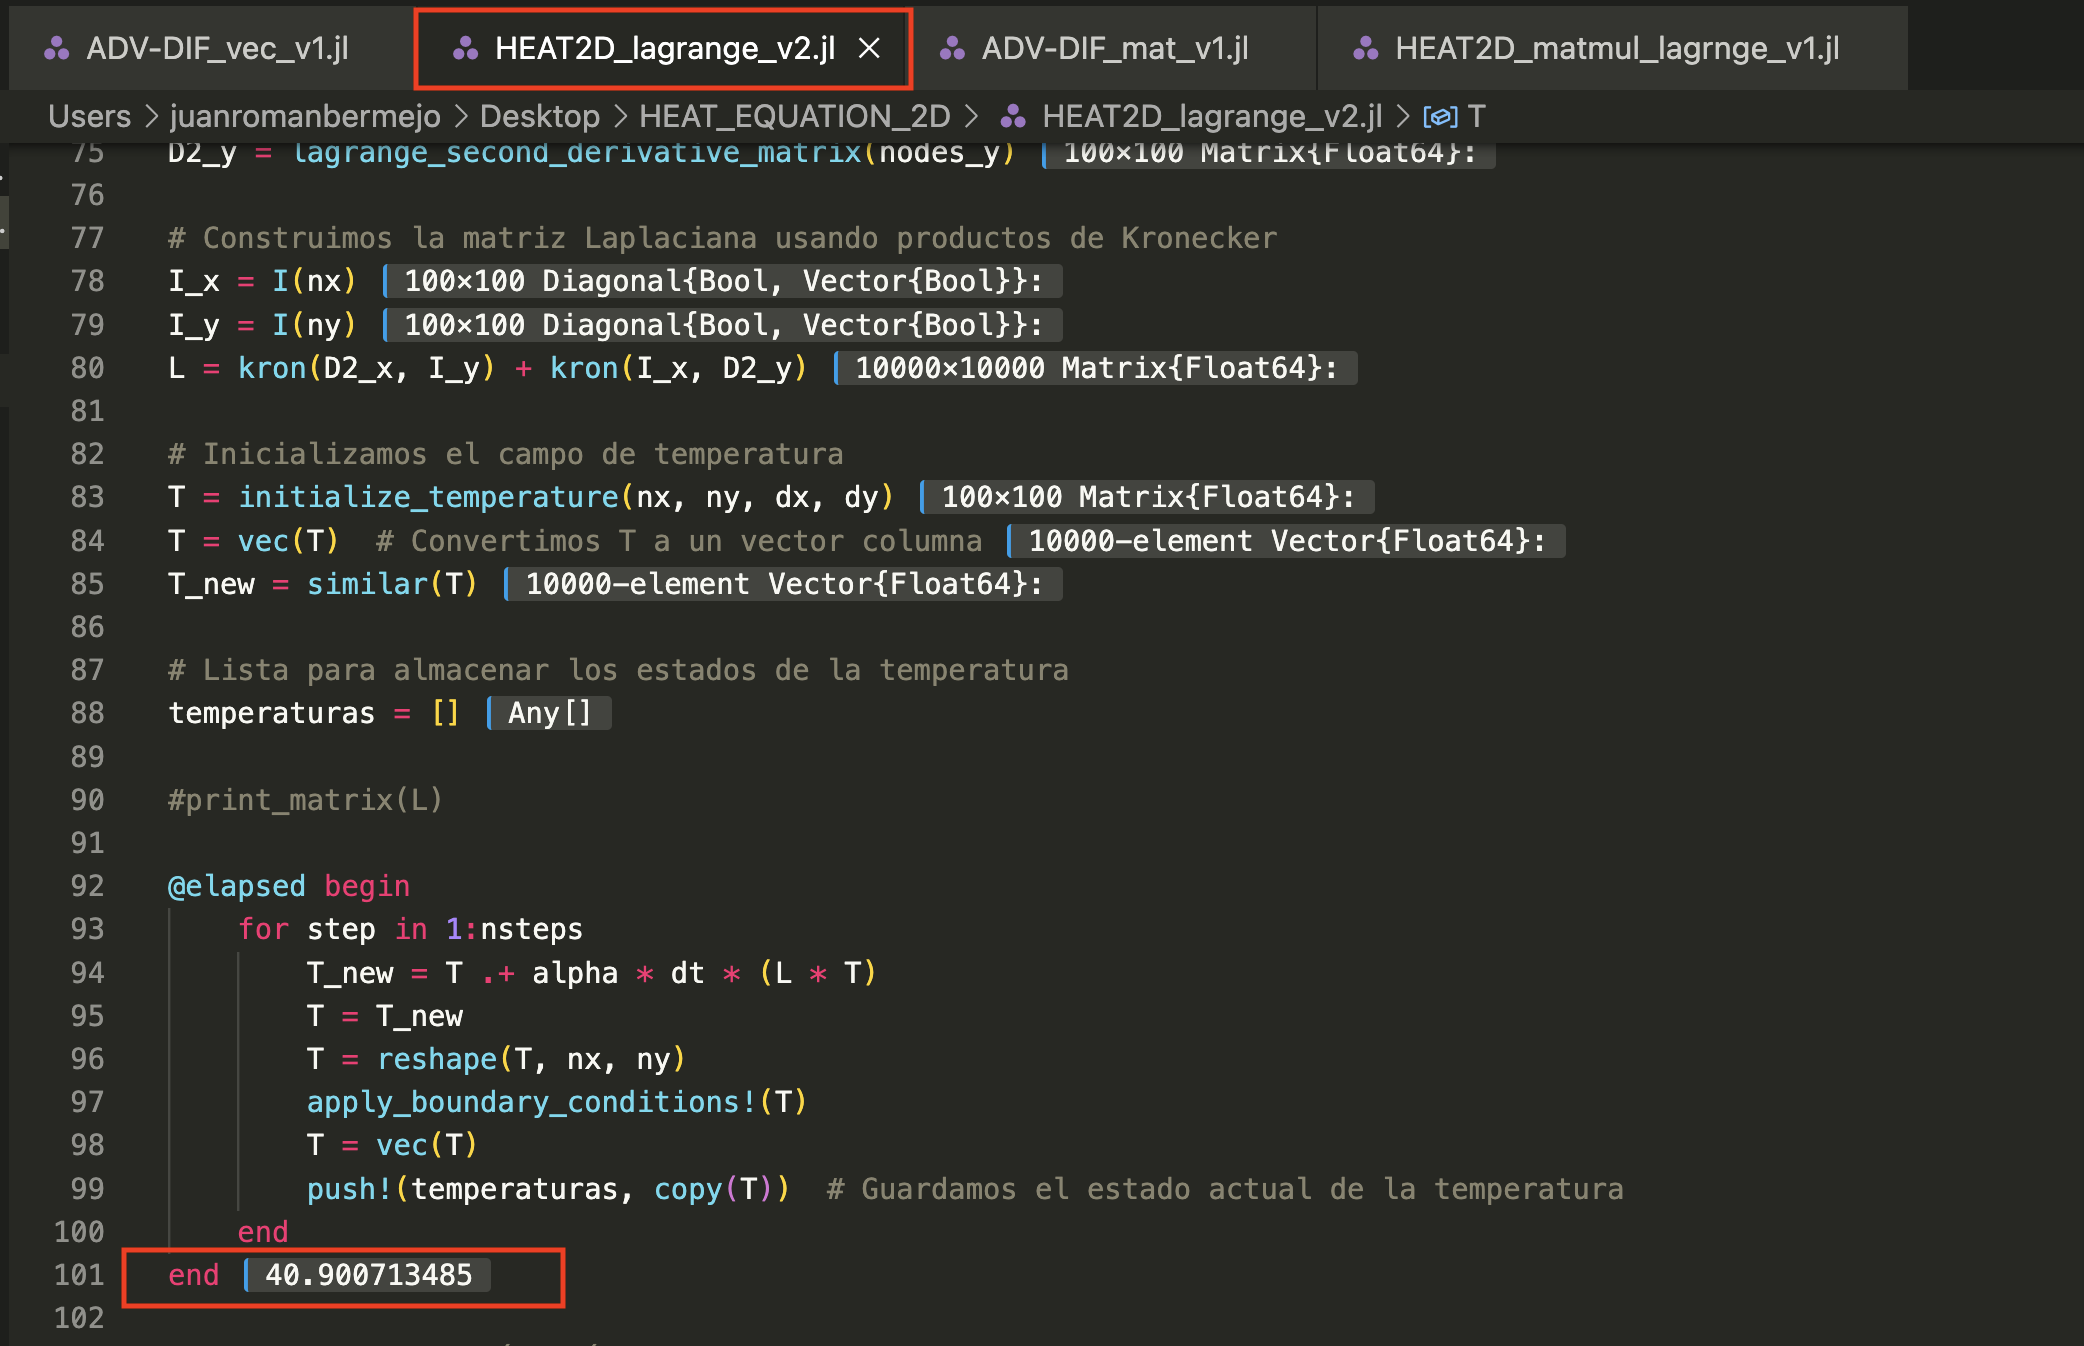
\includegraphics[width=0.7\textwidth]{Figures/HEAT-VEC-time.png}
    \caption{ Matrix-vector}
    \label{fig:etiqueta_figure}
\end{figure}


\begin{figure}[H]
    \centering
    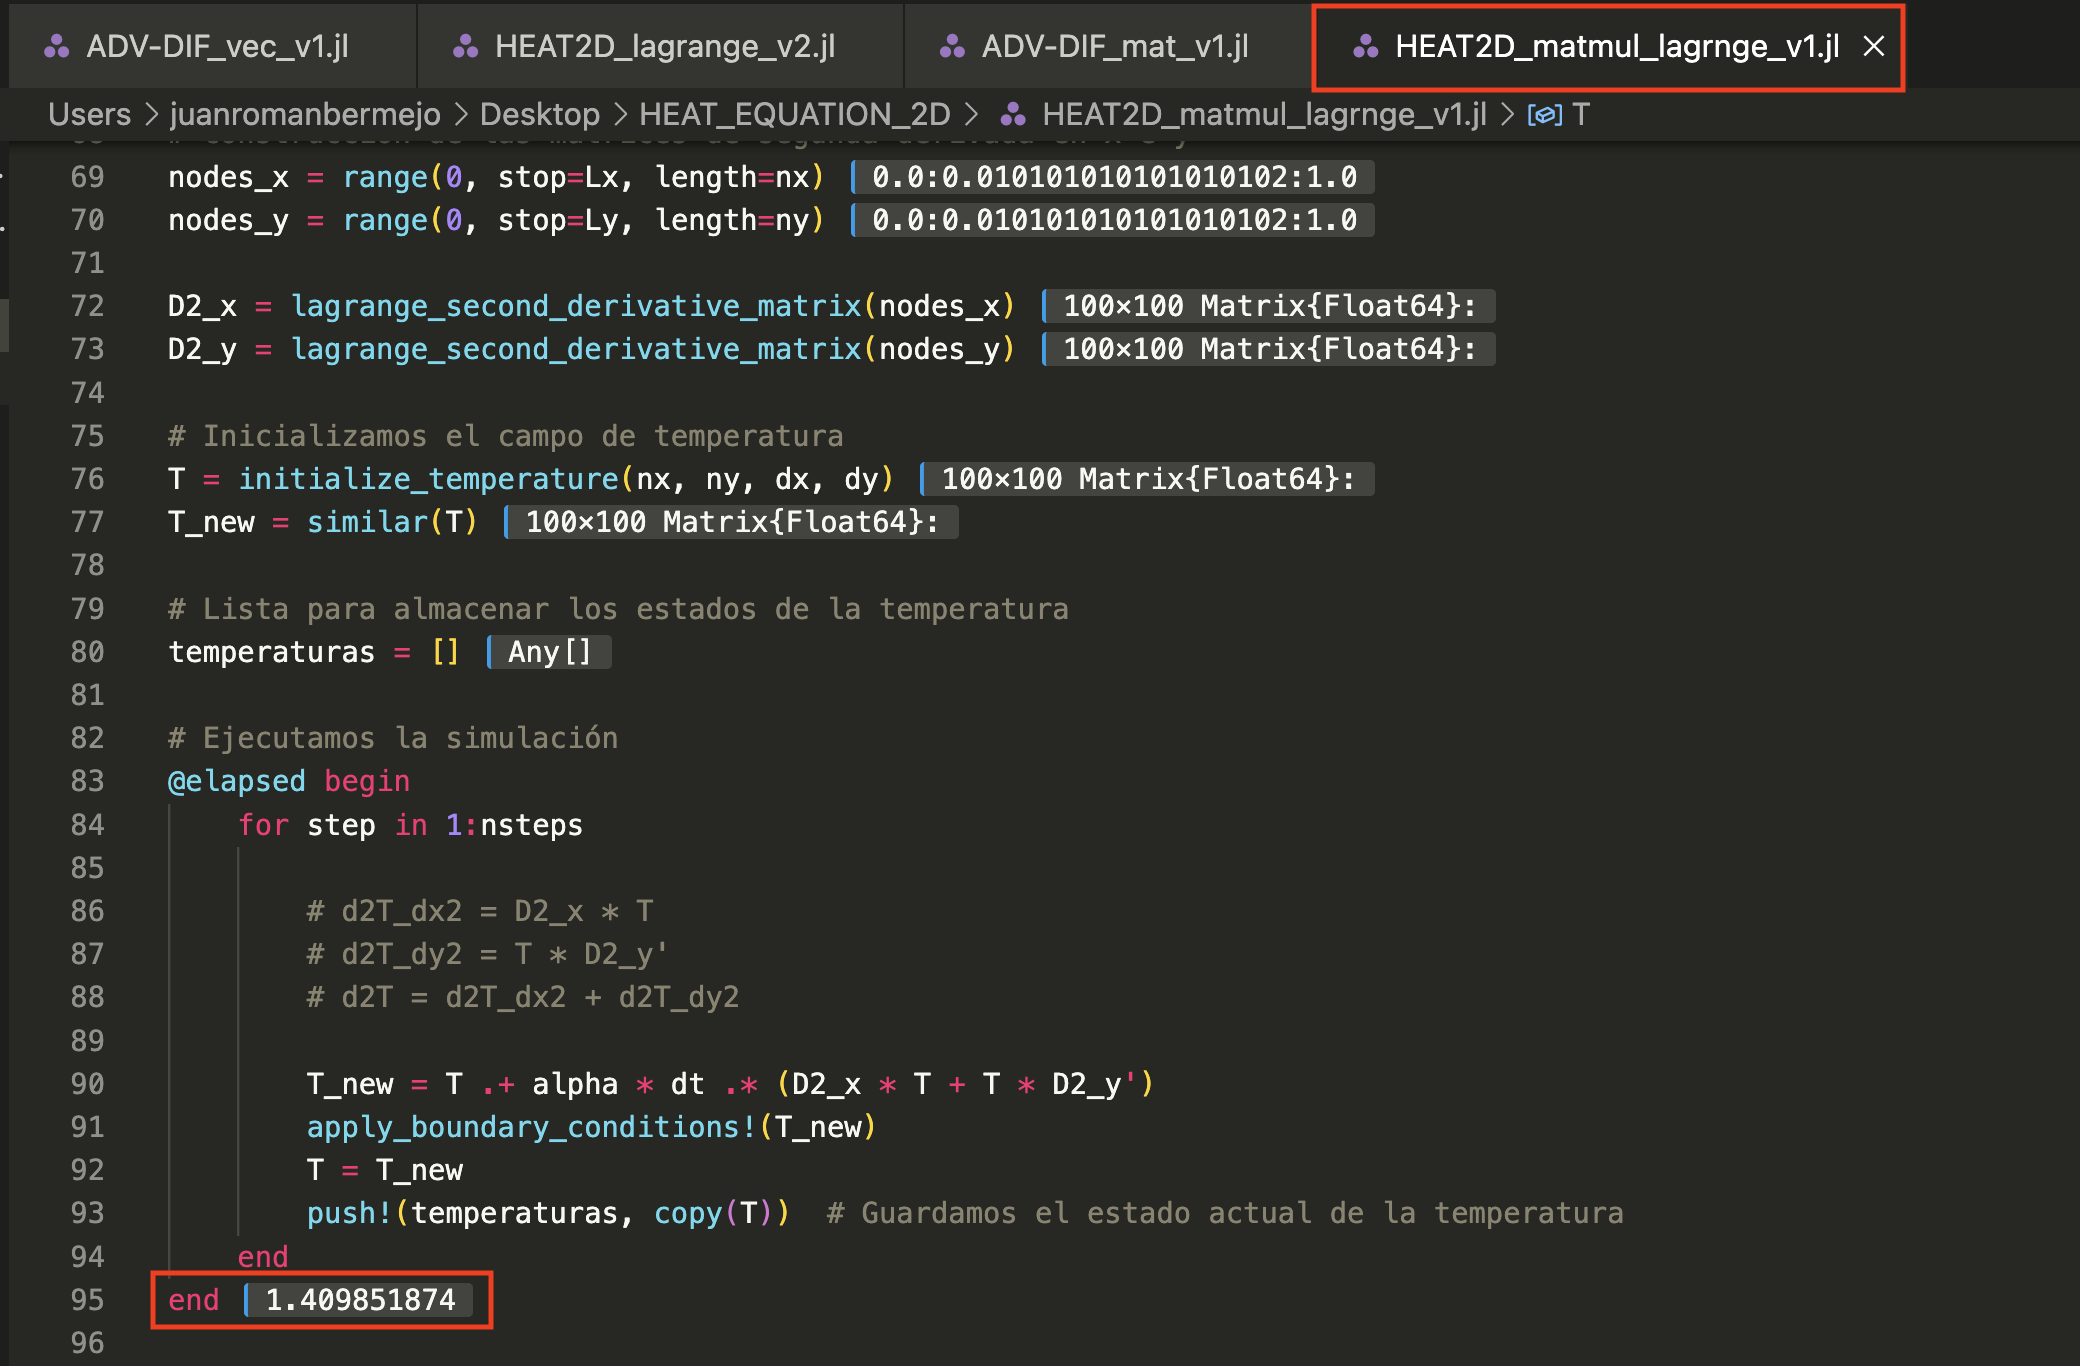
\includegraphics[width=0.7\textwidth]{Figures/HEAT-MAT-time.png}
    \caption{Matriz por Matriz}
    \label{fig:etiqueta_figure}
\end{figure}


\newpage
The results are the following: 


\begin{figure}[h!]
    \centering
    \begin{minipage}[b]{0.3\textwidth}
        \centering
        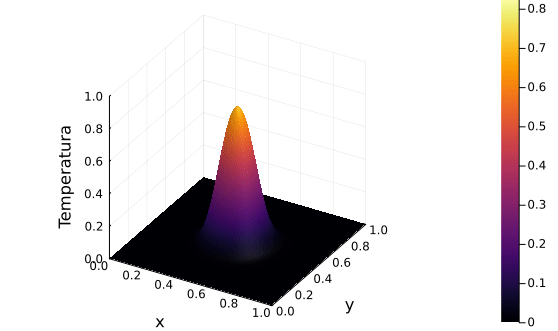
\includegraphics[width=\textwidth]{Figures/inicb.png}
        \caption{Image 1}
    \end{minipage}
    \hfill
    \begin{minipage}[b]{0.3\textwidth}
        \centering
        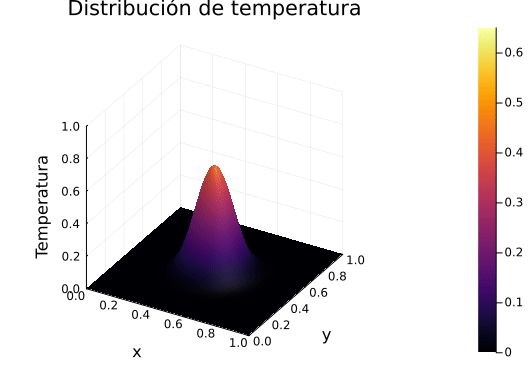
\includegraphics[width=\textwidth]{Figures/inic.png}
        \caption{Image 2}
    \end{minipage}
    \hfill
    \begin{minipage}[b]{0.3\textwidth}
        \centering
        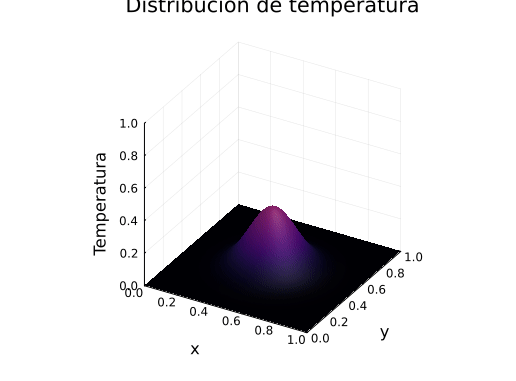
\includegraphics[width=\textwidth]{Figures/end.png}
        \caption{Image 3}
    \end{minipage}
\end{figure}



After these results, we attempted a more complex simulation, where we observed the evolution of the temperature around a rectangle at a constant temperature $T_{\text{const}}$, immersed in a flow with a different ambient temperature $T_{\infty}$ and a uniform velocity. The first test is done using finite differences, as shown in the figure below(t=0.416):


\begin{figure}[H]
    \centering
    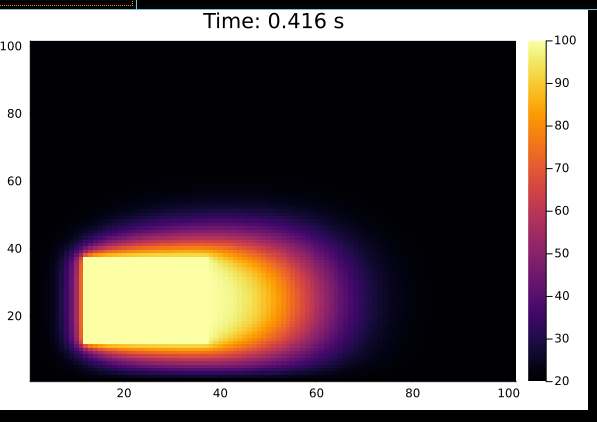
\includegraphics[width=0.7\textwidth]{Figures/rect2.png}
    \caption{Heat distribution around rectangle (t=0.416)}
    \label{fig:etiqueta_figure}
\end{figure}

\newpage 
The code used for this is the following:


\begin{lstlisting}[language=Julia]
using Plots
using Printf

# Parameters
nx, ny = 100, 100       # numero de puntos en x e y
Lx, Ly = 1.0, 1.0       # dimensiones del dominio
dx, dy = Lx/nx, Ly/ny   # espaciado de la malla
alpha = 0.01        # difusividad termica
T_inf = 20.0            # temperatura del aire entrante
T_rect = 100.0          # temperatura del rectangulo
u = 0.1            # velocidad del flujo de aire (izquierda a derecha)

# Esabilidad usando CFL 
dt_diff = (dx^2) / (2 * alpha)
dt_conv = dx / u
dt_max = min(dt_diff, dt_conv)
dt = min(dt_max, 0.0001)  # elegir dt estable

println("Paso temporal: $dt")
println("Maximo paso estable: $dt_max")

# Numero de pasos
t_end = 1.0             # tiempo final
nsteps = Int(t_end / dt)

# Inicializacion del campo de temperatura
T = fill(T_inf, nx+1, ny+1)

# Indices del rectangulo
rect_x = Int(floor(nx/8)):Int(floor(3*nx/8))
rect_y = Int(floor(ny/8)):Int(floor(3*ny/8))
T[rect_x, rect_y] .= T_rect

# Condiciones de contorno
function apply_boundary_conditions!(T, T_inf, u, dt, dx)
    nx, ny = size(T)
    
    # Inflow (left side)
    T[1, :] .= T_inf
    
    # Outflow (right side) - COND CONT Convectiva outflow 
   # for j in 1:ny
   #     T[end, j] = T[end, j] - u * dt / dx * (T[end, j] - T[end-1, j])
    #end
    
    



    # Arriba 
    T[:, end] .= T_inf
    
    # Abajo 
    T[:, 1] .= T_inf
end

# Actualizar el campo de temperatura
function update_temperature!(T, alpha, u, dx, dy, dt)
    nx, ny = size(T)
    T_new = copy(T)
    for i in 2:nx-1
        for j in 2:ny-1
            # Conveccion
            convection = -u * (T[i,j] - T[i-1,j]) / dx
 #upwinding
 
 # Tx = Dx T  Incluye todas las derivadas (cualquier orden) ver Matvect/ matmat// para ver comparacion(tiempo y resultados) u*gradT
            # Difusion

            # Txx = Dxx T igual evaluar que implementacion va mas rapido Dxx la calculas una vez 

            diffusion = alpha * (
                (T[i+1,j] - 2*T[i,j] + T[i-1,j]) / dx^2 +
                (T[i,j+1] - 2*T[i,j] + T[i,j-1]) / dy^2 )
            
            T_new[i,j] = T[i,j] + dt * (convection + diffusion)
        end
    end
    return T_new
end

# Temperatura del rectangulo
function set_rectangle_temperature!(T, rect_x, rect_y, T_rect)
    T[rect_x, rect_y] .= T_rect
end

# Configuracion de la visualizacion
anim = Animation()

# Bucle de integracion en el tiempo
for step in 1:nsteps
    # Aplicar condiciones de contorno
    apply_boundary_conditions!(T, T_inf, u, dt, dx)

    # Actualizar el campo de temperatura
    global T = update_temperature!(T, alpha, u, dx, dy, dt)

    # Fijar la temperatura del rectangulo
    set_rectangle_temperature!(T, rect_x, rect_y, T_rect)

    # Visualizacion
    if step % 10 == 0
        heatmap(T', c=:inferno, clim=(T_inf, T_rect), title=@sprintf("Time: %.3f s", step*dt))
        frame(anim)
    end
end

# Guardar la animacion como GIF
gif(anim, "heat_transfer_simulation1.gif", fps=10)

\end{lstlisting}
